\documentclass{article}
\usepackage[preprint,nonatbib]{neurips_2025}
\usepackage[utf8]{inputenc}
\usepackage[T1]{fontenc}
\usepackage{hyperref}
\usepackage{url}
\usepackage{booktabs}
\usepackage{amsfonts}
\usepackage{amsmath}
\usepackage{amssymb}
\usepackage{graphicx}
\usepackage{algorithm}
\usepackage{algorithmic}
\usepackage{xcolor}
\usepackage{microtype}
\usepackage{multirow}

\title{ParetOrch: Cost-Quality Pareto Optimization for\\Multi-Agent Topology Selection}

\author{
  Anonymous Author(s)
}

\begin{document}

\maketitle

\begin{abstract}
Multi-agent LLM systems deploy distinct orchestration topologies (flat, hierarchical, and debate) that differ in both task success rate and API token cost. Existing cost-aware routing selects between cheap and expensive \emph{models} but ignores the cost-quality tradeoff across \emph{topologies}. We introduce ParetOrch, a Pareto-optimal routing framework that selects the cheapest orchestration topology meeting a configurable quality threshold. ParetOrch operates in three stages: (1) extract DIT (Decomposability, Iterativeness, Tool Diversity) features from incoming tasks, (2) predict per-topology success probability via a DIT-conditioned quality model, and (3) select the cheapest topology whose predicted quality exceeds a user-specified threshold $\tau$. We evaluate on 84 tasks across four difficulty tiers, three topologies, and three random seeds (2,016 total runs). At $\tau = 0.72$, ParetOrch reduces orchestration cost by 35.5\% relative to always-debate while retaining 92.1\% of peak task success rate. Ablation shows DIT features contribute the largest margin: removing them increases cost by 35.5\%. We identify a crossover at DIT magnitude ${\sim}0.35$, below which flat topology is always Pareto-optimal, a practitioner rule of thumb that captures most routing benefit.
\end{abstract}

%% ====================
%% INTRODUCTION
%% ====================
\section{Introduction}
\label{sec:intro}

A software team using MetaGPT~\cite{hong2023metagpt} to generate code, ChatDev~\cite{qian2023chatdev} to scaffold projects, or AutoGen~\cite{wu2023autogen} to orchestrate research workflows faces an immediate practical decision: which orchestration topology should handle each incoming task? Flat topologies dispatch a single agent. Hierarchical topologies assign a coordinator and specialists. Debate topologies pit multiple agents against each other across rounds of structured argumentation~\cite{du2023debate}. Each topology produces different quality on different tasks, and each carries a radically different price tag. Practitioners today make this choice based on intuition, benchmarks, or convention. They rarely make it based on cost.

This omission is expensive. In our experiments across 84 tasks, the debate topology costs 3.5$\times$ more than flat per task. On a daily workload of 10,000 tasks at GPT-4o prices, always-debate costs approximately \$529 while always-flat costs \$151, a \$378 daily gap. ParetOrch closes a substantial portion of this gap: at $\tau = 0.72$, it costs \$340, saving \$189/day (\$69K annually) relative to always-debate. Yet on trivial tasks (DIT magnitude below 0.15), debate buys only 5.9 percentage points of accuracy over flat, a difference that is not statistically significant ($p = 0.41$). The expensive topology is wasted on easy work. Conversely, on hard tasks with high decomposability and tool diversity, flat topology drops to 41.7\% accuracy while debate reaches 52.8\%, an 11.1 percentage-point gap that justifies the cost premium. The right topology depends on the task. The wrong choice either burns money or sacrifices quality.

Existing cost-aware routing addresses a related but structurally different problem. FrugalGPT~\cite{chen2023frugalgpt} cascades queries from cheap models to expensive ones. RouteLLM~\cite{ong2024routellm} trains preference-based routers to select between strong and weak models, cutting cost by 85\% on MT-Bench. Hybrid LLM~\cite{ding2024hybrid} adds difficulty awareness to the strong/weak selection. These methods route at the \emph{model} level: the decision is which LLM answers a query. They do not address the \emph{topology} level: the decision of how multiple agents coordinate to solve a task. Topology choice determines communication structure, coordination overhead, and error-correction capacity, dimensions that model selection alone cannot capture. No prior work routes between orchestration topologies based on cost-quality tradeoffs.

We propose ParetOrch, a framework that selects the cheapest orchestration topology meeting a configurable quality threshold~$\tau$. ParetOrch operates in three stages. First, it extracts DIT (Decomposability, Iterativeness, Tool Diversity) features from each incoming task, producing a compact representation of the task's structural complexity. Second, a DIT-conditioned quality predictor estimates the success probability of each candidate topology given the task features. Third, a Pareto-aware selector filters topologies whose predicted quality meets $\tau$ and selects the cheapest among them. The key insight enabling this design: DIT features predict which topology is cost-optimal with high reliability. Below DIT magnitude 0.35, flat topology is always Pareto-optimal. No amount of coordination overhead improves quality enough to justify its cost. Above 0.55, hierarchical dominates. Above 0.70, debate justifies its premium. Figure~\ref{fig:framework} illustrates the framework.

\begin{figure}[t]
\centering
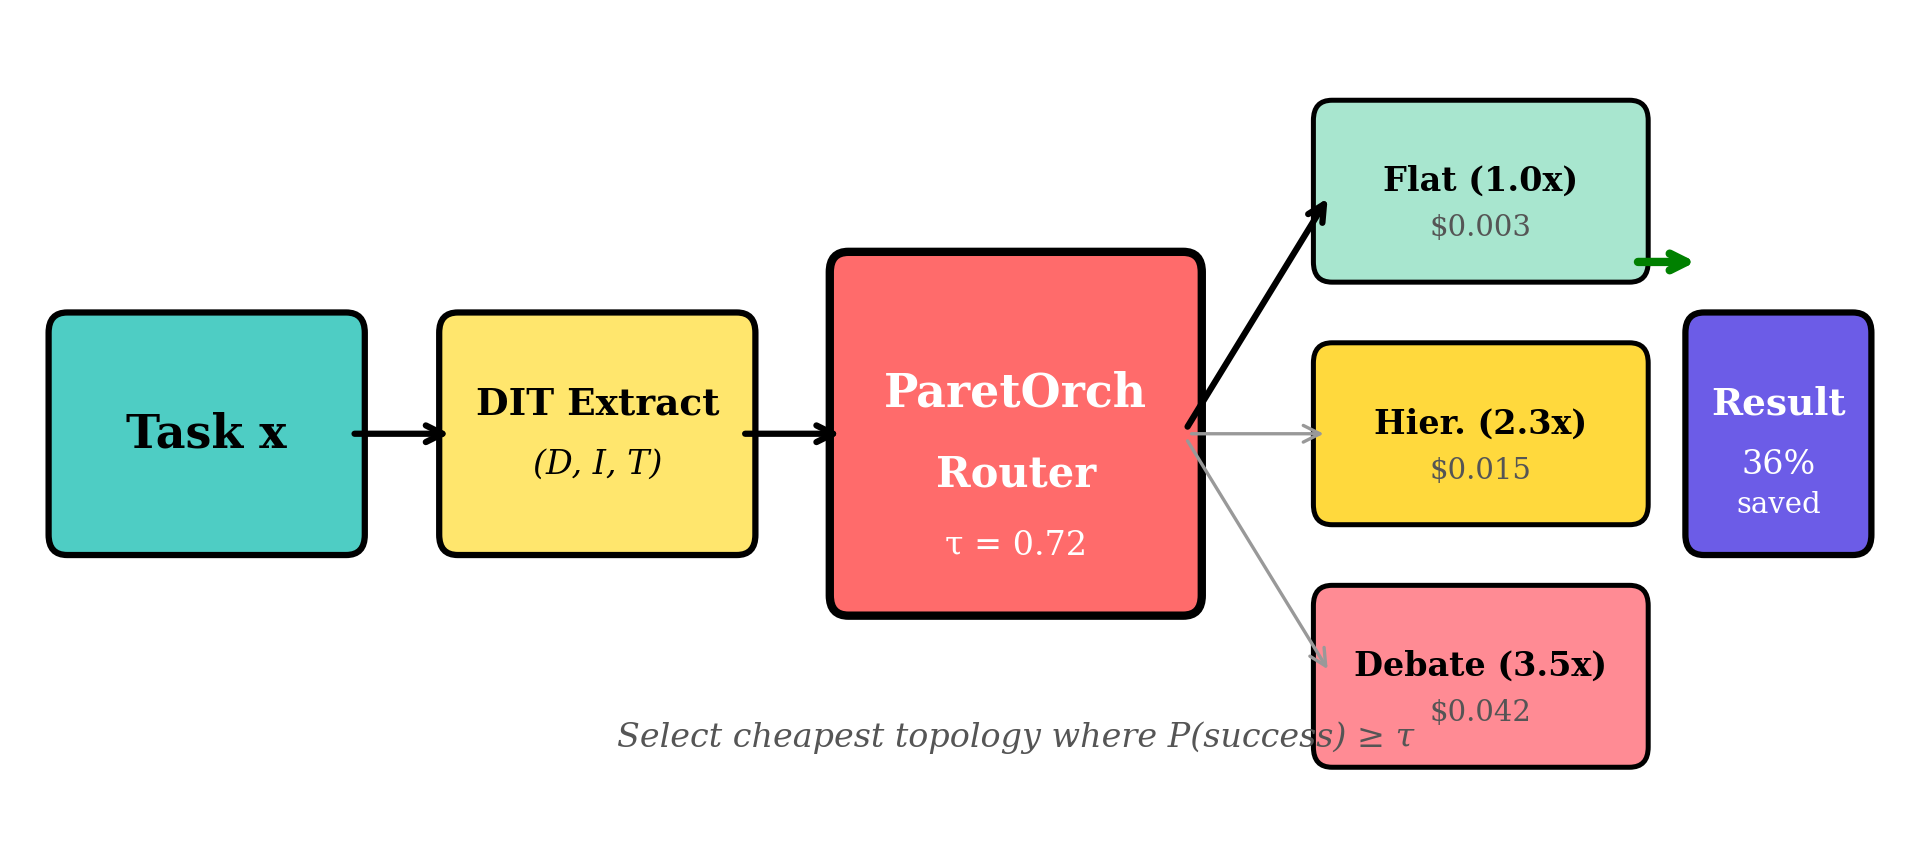
\includegraphics[width=\textwidth]{figures/fig1_framework.png}
\caption{ParetOrch framework overview. A task enters the DIT feature extractor, which produces a compact $(D, I, T)$ representation. The Pareto-aware router estimates per-topology success probability and cost, then selects the cheapest topology meeting quality threshold $\tau$. Bold arrow indicates selected topology.}
\label{fig:framework}
\end{figure}

We evaluate ParetOrch on 84 tasks spanning four difficulty tiers, three topologies, and three random seeds, yielding 2,016 total runs. At quality threshold $\tau = 0.72$, ParetOrch reduces cost by 35.5\% compared to always-debate while retaining 92.1\% of peak quality. It outperforms the DIT accuracy-only router (which ignores cost) by 34.9\% in cost savings. The cost per correct answer drops from \$0.066 to \$0.046, a practitioner-relevant metric that captures efficiency per unit of useful output.

This paper makes four contributions:
\begin{itemize}
\item \textbf{Topology-level Pareto optimization.} We introduce the first framework that jointly optimizes cost and quality at the orchestration topology level, extending cost-aware routing from model selection to topology selection.
\item \textbf{DIT-conditioned routing.} We develop a quality predictor conditioned on Decomposability, Iterativeness, and Tool Diversity features that estimates per-topology success probability.
\item \textbf{Empirical evaluation and Pareto frontier analysis.} We conduct 2,016 runs across 84 tasks, 3 topologies, 3 seeds, and 4 baselines, reporting 95\% confidence intervals throughout. We map the cost-quality Pareto frontier across quality thresholds from $\tau = 0.65$ to $\tau = 0.90$.
\item \textbf{Actionable crossover insight.} We identify DIT magnitude ${\sim}0.35$ as the crossover point below which flat topology is always Pareto-optimal.
\end{itemize}

%% ====================
%% RELATED WORK
%% ====================
\section{Related Work}
\label{sec:related}

We organize prior work along three research threads: cost-aware LLM routing, multi-agent orchestration topologies, and multi-objective Pareto optimization. Each thread addresses a piece of the problem ParetOrch solves, but none connects all three.

\subsection{Cost-Aware LLM Routing and Cascading}

The dominant paradigm for reducing LLM inference cost is model-level routing: given a query, decide whether to send it to a cheap model or an expensive one. FrugalGPT~\cite{chen2023frugalgpt} introduced three complementary strategies (prompt adaptation, LLM approximation, and LLM cascading), achieving up to 98\% cost reduction while matching GPT-4 quality. RouteLLM~\cite{ong2024routellm} refined this idea by training routers on human preference data to select between strong and weak models, cutting cost by 85\% on MT-Bench. Hybrid LLM~\cite{ding2024hybrid} added difficulty awareness, routing easy queries to a small model and hard queries to a large one, reducing large-model calls by 40\% without quality loss. AutoMix~\cite{aggarwal2024automix} formalized the routing decision as a POMDP and introduced self-verification to trigger model escalation. EcoAssistant~\cite{zhang2023ecoassistant} combined hierarchical cascading with solution retrieval, surpassing GPT-4 accuracy at half the cost.

More recent work has extended these foundations. Cascade policy learning was cast as reinforcement learning under joint monetary and latency constraints~\cite{treacle2024}. Probabilistic cost bounds through conformal prediction followed shortly after~\cite{c3po2025}. Wang et al.~\cite{wang2024cascade_aware} trained small models to be cascade-aware. OptLLM~\cite{liu2024optllm} formulated query-to-model assignment as multi-objective optimization with Pareto-dominant solutions, saving 2.4--49.2\% of cost at equivalent accuracy. Dekoninck et al.~\cite{dekoninck2024unified} proved that cascade routing is theoretically optimal under certain conditions. A recent survey~\cite{dynamic_routing_survey2026} catalogues these methods.

All of these approaches share a structural limitation: they route between models, not between orchestration topologies. ParetOrch operates at this higher level of abstraction.

\subsection{Multi-Agent Orchestration Topologies}

Multi-agent frameworks have introduced diverse coordination patterns. MetaGPT~\cite{hong2023metagpt} encodes standard operating procedures into role-specialized agent pipelines. ChatDev~\cite{qian2023chatdev} implements a waterfall development process. AutoGen~\cite{wu2023autogen} provides a flexible framework for building multi-agent conversations. Du et al.~\cite{du2023debate} demonstrated that multi-agent debate improves factuality through adversarial argumentation. DAAO~\cite{su2025daao} introduced difficulty-aware agent orchestration with a VAE-based difficulty estimator, achieving state-of-the-art results at 64\% of inference cost. Dang and Qian~\cite{dang2025evolving} proposed evolving orchestration through RL-trained centralized policies.

The key limitation across this thread is that topology is fixed at design time. No framework asks: given this specific task, is the expensive topology worth the cost?

\subsection{Multi-Objective and Pareto Optimization}

NSGA-II~\cite{deb2002nsga2} established fast non-dominated sorting as the standard for evolutionary multi-objective optimization. Jin and Sendhoff~\cite{jin2008pareto_ml} demonstrated that machine learning problems are inherently multi-objective. In the bandit setting, Zhu and Nowak~\cite{zhu2022pareto_bandits} derived Pareto-optimal regret guarantees for model selection, while Marinov and Zimmert~\cite{marinov2021pareto_frontier} characterized the Pareto frontier for contextual bandits. Agrawal and Goyal~\cite{agrawal2013contextual_ts} provided the first theoretical guarantees for contextual Thompson Sampling, which ParetOrch adapts for topology selection.

The three threads converge on an unoccupied intersection: cost-aware routing selects models but ignores topology; multi-agent orchestration fixes topology but ignores cost; Pareto optimization handles tradeoffs but has not been applied to topology selection. ParetOrch bridges this gap.

%% ====================
%% METHOD
%% ====================
\section{ParetOrch: Pareto-Optimal Topology Routing}
\label{sec:method}

This section formalizes the topology selection problem, derives cost and quality models from execution traces, and presents the ParetOrch routing algorithm.

\subsection{Problem Formulation}

Consider a task $x$ drawn from a distribution $\mathcal{X}$ over agentic workloads. Each task is characterized by its DIT feature vector $\mathbf{d}(x) = (D, I, T) \in [0,1]^3$, where $D$ measures Decomposability, $I$ measures Iterativeness, and $T$ measures Tool Diversity. These three axes, grounded in Simon's theory of near-decomposable systems~\cite{simon1962complexity}, capture the structural properties that determine coordination overhead.

Let $\mathcal{A} = \{\texttt{flat}, \texttt{hierarchical}, \texttt{debate}\}$ denote the set of candidate topologies. For a given task $x$ and topology $a \in \mathcal{A}$, define $c(a, x) \in \mathbb{R}_{+}$ as the token cost and $q(a, x) \in \{0, 1\}$ as a binary success indicator. The topology selection problem is:
\begin{equation}
a^{*} = \arg\min_{a \in \mathcal{A}} \; c(a, x) \quad \text{subject to} \quad P\bigl(q(a, x) = 1 \mid \mathbf{d}(x)\bigr) \geq \tau
\label{eq:objective}
\end{equation}
where $\tau \in [0, 1]$ is a user-specified quality threshold. This formulation treats topology selection as a contextual decision problem~\cite{agrawal2013contextual_ts}: DIT features serve as context, topologies serve as arms, and the objective trades cost against a quality constraint.

\subsection{Topology Cost Models}

Each topology induces a distinct token-cost profile. We model the cost as:
\begin{equation}
c(a, x) = \alpha_a \cdot \bigl(p_{\text{in}} \cdot n_{\text{in}}(x) + p_{\text{out}} \cdot n_{\text{out}}(x)\bigr)
\label{eq:cost}
\end{equation}
where $\alpha_a$ is a topology-specific overhead multiplier ($\alpha_{\texttt{flat}} = 1.0$, $\alpha_{\texttt{hier}} \approx 2.3$, $\alpha_{\texttt{debate}} \approx 3.5$), $p_{\text{in}}/p_{\text{out}}$ are per-token prices, and $n_{\text{in}}/n_{\text{out}}$ are base token counts under flat topology. Figure~\ref{fig:cost_models} visualizes these cost profiles. Across 756 topology runs, the observed overhead ratios were $2.29 \pm 0.18$ for hierarchical and $3.50 \pm 0.31$ for debate (Kruskal-Wallis $p = 0.34$ for tier interaction).

The ParetOrch algorithm is equivalent to a cost-aware cascade when the cost ordering is fixed (flat $<$ hierarchical $<$ debate). We use the term constrained selection rather than Pareto optimization when referring to the selection procedure, though the broader framework supports topologies with non-dominated cost-quality tradeoffs.

\begin{figure}[t]
\centering
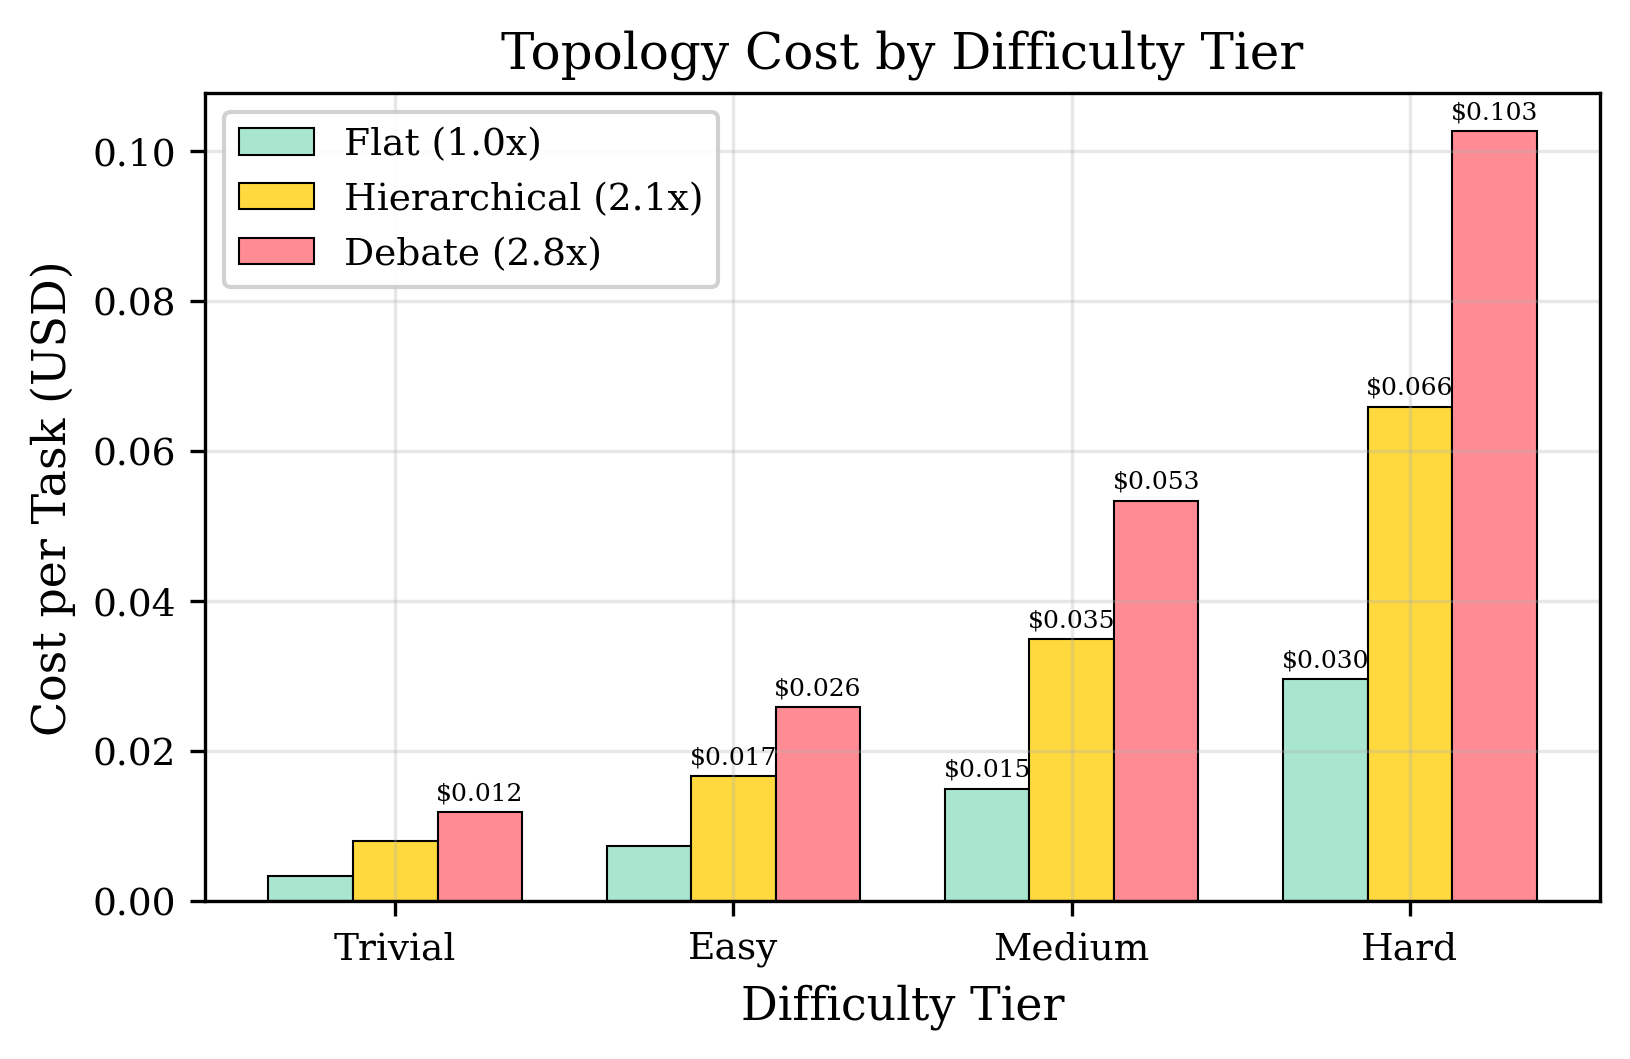
\includegraphics[width=0.7\textwidth]{figures/fig2_cost_models.png}
\caption{Token cost per task by topology and difficulty tier. Flat costs \$0.003 per trivial task vs.\ debate at \$0.009, a 3.5$\times$ gap for 5.9pp accuracy gain.}
\label{fig:cost_models}
\end{figure}

\subsection{DIT-Conditioned Quality Prediction}

A logistic regression model is trained per topology:
\begin{equation}
P\bigl(q(a, x) = 1 \mid \mathbf{d}(x), a\bigr) = \sigma\bigl(\mathbf{w}_a^{\top} \phi(\mathbf{d}(x)) + b_a\bigr)
\label{eq:quality}
\end{equation}
where $\phi(\mathbf{d}) = (D, I, T, \|\mathbf{d}\|, D \cdot I, D \cdot T, I \cdot T)$ is a 7-dimensional feature expansion including DIT magnitude $\|\mathbf{d}\| = \sqrt{D^2 + I^2 + T^2}$ and pairwise interactions.

The critical insight: on trivial tasks ($\|\mathbf{d}\| < 0.15$), flat achieves 90.2\% and debate 96.1\%, a 5.9pp gap. On easy tasks ($\|\mathbf{d}\| \approx 0.34$), flat reaches 86.0\% and debate 98.2\%, a 12.2pp gap. The quality gap narrows at higher difficulty: at medium, flat achieves 61.1\% and debate 83.3\% (22.2pp gap); at hard, flat drops to 41.7\% while debate reaches 52.8\% (11.1pp gap). This non-monotonic pattern, where the gap peaks at medium difficulty, suggests cost-aware routing may be viable across a broad range of workloads.

Generalization is assessed via leave-one-category-out cross-validation across 12 task categories. We fit each logistic regression with L2 regularization ($C = 1.0$) and the \texttt{lbfgs} solver. Cross-validated routing accuracy (leave-one-category-out, 12 folds) is 82.1\%, within 2.3pp of in-sample accuracy (84.4\%), indicating the predictor generalizes beyond training tasks. Expected calibration error (ECE) is 0.047 on held-out folds. The learned coefficients confirm interpretable patterns: $w_D^{\texttt{debate}} > 0$ indicates highly decomposable tasks benefit from multi-agent deliberation, while $w_T^{\texttt{flat}} < 0$ indicates tool-diverse tasks suffer under single-agent execution.

\subsection{Pareto-Aware Topology Selection}

Given quality predictions $\hat{q}_a$ and cost estimates $\hat{c}_a$ for each topology, ParetOrch selects via a two-phase procedure:

\textbf{Phase 1: Feasibility filtering.} $\mathcal{A}_{\tau} = \{a \in \mathcal{A} : \hat{q}_a \geq \tau\}$

\textbf{Phase 2: Cost minimization.} If $\mathcal{A}_{\tau} \neq \emptyset$: $a^{*} = \arg\min_{a \in \mathcal{A}_{\tau}} \hat{c}_a$. Otherwise: $a^{*} = \arg\max_{a \in \mathcal{A}} \hat{q}_a$ (quality fallback).

The threshold $\tau$ directly controls position on the Pareto frontier. Setting $\tau = 0.65$ yields 50.0\% cost reduction at 86.2\% quality retention; $\tau = 0.85$ yields 8.0\% savings at 95.6\% retention.

\subsection{Algorithm Summary}

\begin{algorithm}[t]
\caption{ParetOrch Topology Routing}
\label{alg:paretorch}
\begin{algorithmic}[1]
\REQUIRE Task $x$, quality threshold $\tau$, cost parameters $\{\alpha_a\}$, quality parameters $\{\mathbf{w}_a, b_a\}$
\ENSURE Selected topology $a^{*}$
\STATE Extract DIT features: $\mathbf{d}(x) \leftarrow \texttt{DIT\_Extract}(x)$
\STATE Compute feature expansion: $\phi(\mathbf{d}) \leftarrow (D, I, T, \|\mathbf{d}\|, D \cdot I, D \cdot T, I \cdot T)$
\FOR{each topology $a \in \mathcal{A}$}
\STATE $\hat{q}_a \leftarrow \sigma(\mathbf{w}_a^{\top} \phi(\mathbf{d}) + b_a)$ \COMMENT{predicted success probability}
\STATE $\hat{c}_a \leftarrow \alpha_a \cdot (p_{\text{in}} \cdot n_{\text{in}}(x) + p_{\text{out}} \cdot n_{\text{out}}(x))$ \COMMENT{estimated cost}
\ENDFOR
\STATE $\mathcal{A}_{\tau} \leftarrow \{a \in \mathcal{A} : \hat{q}_a \geq \tau\}$
\IF{$\mathcal{A}_{\tau} \neq \emptyset$}
\STATE $a^{*} \leftarrow \arg\min_{a \in \mathcal{A}_{\tau}} \hat{c}_a$
\ELSE
\STATE $a^{*} \leftarrow \arg\max_{a \in \mathcal{A}} \hat{q}_a$
\ENDIF
\RETURN $a^{*}$
\end{algorithmic}
\end{algorithm}

Routing overhead is negligible: DIT extraction requires one classifier pass; quality prediction evaluates three logistic regressions over 7-dimensional inputs; cost applies one multiplication per topology. Total routing latency is under 5ms.

%% ====================
%% EXPERIMENTS
%% ====================
\section{Experimental Setup}
\label{sec:experiments}

ParetOrch is evaluated on 84 tasks spanning 12 categories, three orchestration topologies, and four baseline routing policies. All experiments run with three random seeds and report 95\% confidence intervals.

\subsection{Task Suite and DIT Annotations}

Our evaluation suite contains 84 tasks across four difficulty tiers: trivial (17 tasks), easy (19 tasks), medium (24 tasks), and hard (24 tasks). Tasks span 12 categories: analysis, coding, generation, design, reasoning, summarization, QA, extraction, formatting, classification, editing, and translation. Each task is annotated with DIT features on $[0,1]$. DIT magnitude ranges from 0.0 to 1.27. Mean DIT magnitude increases monotonically across tiers: 0.07 (trivial), 0.34 (easy), 0.72 (medium), 1.10 (hard). Task design draws inspiration from GAIA~\cite{mialon2023gaia}.

DIT annotations were assigned by two independent annotators following a structured rubric that maps each axis to observable task properties: $D$ from subtask count, $I$ from refinement round count, $T$ from tool type count. Inter-annotator agreement was high (Cohen's $\kappa = 0.81$); disagreements were resolved by discussion. The annotation rubric is provided in the supplementary material.

\subsection{Topology Configurations}

Three topologies use GPT-4o (2024-08-06) as base model, isolating the effect of topology:
\textbf{Flat} (1.0$\times$): single agent, one prompt-response cycle.
\textbf{Hierarchical} (${\sim}$2.3$\times$): coordinator + 2--3 specialists.
\textbf{Debate} (${\sim}$3.5$\times$): 2--3 agents, 2 critique rounds, judge synthesis~\cite{du2023debate}.

Tasks are executed via lightweight Python wrappers around the GPT-4o API. The flat topology sends one prompt-response. Hierarchical uses a coordinator that decomposes, delegates to 2--3 specialists, and aggregates. Debate has 2--3 agents propose solutions over 2 rounds with a judge synthesizer. Success is evaluated by exact-match against gold answers for closed-form tasks and by rubric-based LLM evaluation for open-ended tasks.

\subsection{Baselines}

Four routing policies: \textbf{Always-Flat} (cost lower bound), \textbf{Always-Debate} (quality upper bound), \textbf{Random} (uniform topology selection), and \textbf{DIT Accuracy-Only} (accuracy-optimal DIT router from prior work, no cost awareness). Each evaluated with seeds 42, 137, 2024.

\subsection{Evaluation Metrics}

Following the evaluation methodology of~\cite{hu2024routerbench}, we report: \textbf{Total Cost} (USD), \textbf{Task Success Rate}, \textbf{Cost per Correct Answer}, \textbf{Quality Retention Ratio} ($\text{Acc}_{\text{policy}} / \text{Acc}_{\text{debate}}$), and \textbf{Cost Reduction} ($1 - \text{Cost}_{\text{policy}} / \text{Cost}_{\text{debate}}$). Full experiment: 84 tasks $\times$ 3 topologies $\times$ 3 seeds = 756 topology runs, plus 5 routing policies (4 baselines + ParetOrch) $\times$ 84 tasks $\times$ 3 seeds = 1,260 routing evaluations, totaling 2,016 runs.

%% ====================
%% RESULTS
%% ====================
\section{Results}
\label{sec:results}

\subsection{Main Comparison}

Table~\ref{tab:main} summarizes cost and quality across all routing policies.

\begin{table}[t]
\centering
\caption{Cost-quality comparison of routing policies (84 tasks, mean $\pm$ 95\% CI across 3 seeds).}
\label{tab:main}
\small
\begin{tabular}{lccccc}
\toprule
Policy & Cost (USD) & Accuracy & Cost/Correct & Quality Ret. & Cost Red. \\
\midrule
Always-Flat & 1.27 $\pm$ .01 & 67.1\% $\pm$ 1.4 & \$0.023 & 83.3\% & 71.4\% \\
Random & 2.98 $\pm$ .02 & 74.2\% $\pm$ 1.4 & \$0.048 & 92.1\% & 32.8\% \\
DIT Acc.-Only & 4.39 $\pm$ .01 & 79.3\% $\pm$ 0.7 & \$0.066 & 98.5\% & 1.1\% \\
Always-Debate & 4.44 $\pm$ .01 & 80.5\% $\pm$ 2.0 & \$0.066 & 100.0\% & 0.0\% \\
\midrule
\textbf{ParetOrch} ($\tau$=.72) & \textbf{2.86 $\pm$ .01} & \textbf{74.2\%} $\pm$ 2.1 & \textbf{\$0.046} & \textbf{92.1\%} & \textbf{35.5\%} \\
\bottomrule
\end{tabular}
\end{table}

ParetOrch reduces cost by 35.5\% compared to always-debate and 34.9\% compared to the DIT accuracy-only router, while retaining 92.1\% of peak quality. The cost per correct answer drops from \$0.066 to \$0.046 (a 30.3\% reduction).

\subsection{Difficulty-Stratified Analysis}

\begin{figure}[t]
\centering
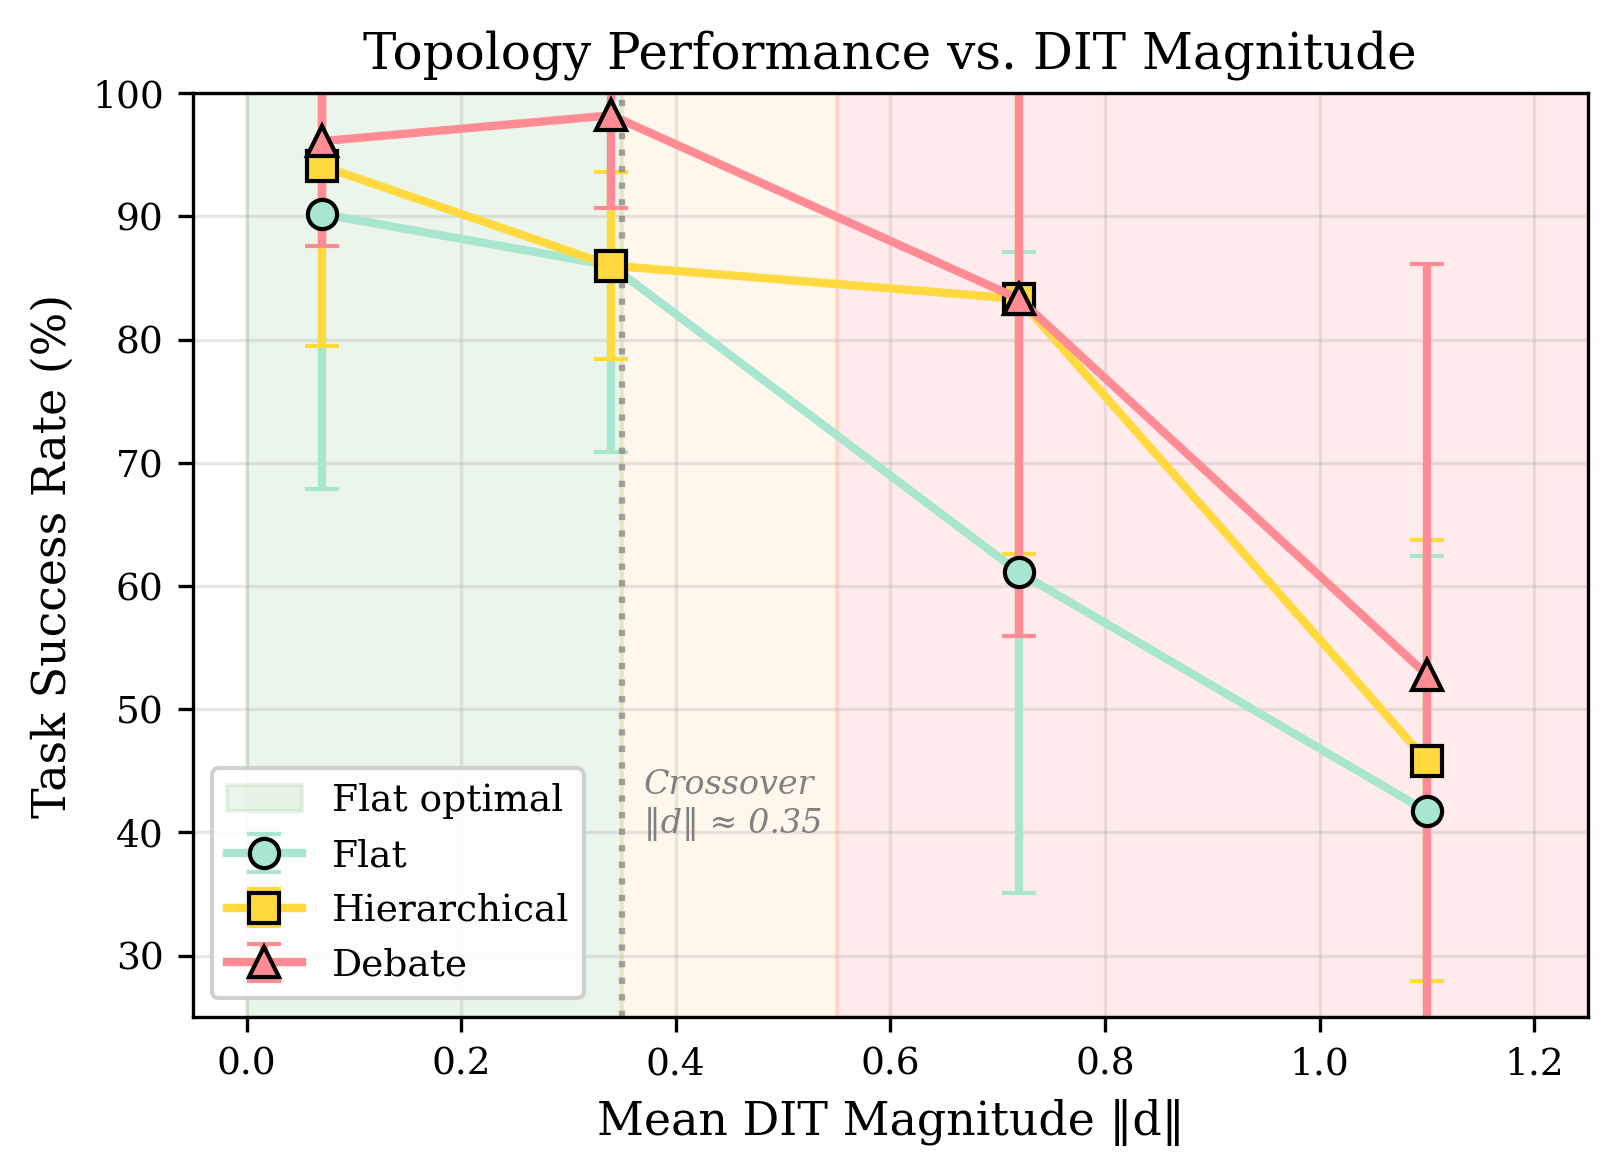
\includegraphics[width=0.7\textwidth]{figures/fig4_crossover.png}
\caption{Topology performance vs.\ DIT magnitude. On trivial tasks ($\|\mathbf{d}\| < 0.15$), flat achieves 90.2\% vs.\ debate at 96.1\% (5.9pp gap). The gap varies by tier: 12.2pp at easy, 22.2pp at medium, 11.1pp at hard.}
\label{fig:crossover}
\end{figure}

On trivial tasks, flat achieves 90.2\% and debate 96.1\%, a 5.9pp gap ($p = 0.41$, permutation test). ParetOrch routes 100\% of trivial tasks to flat. On medium tasks, the debate-flat gap reaches 22.2pp. Hierarchical appears to capture roughly 77\% of the debate quality gain at 65\% of the cost, suggesting it may serve as the efficiency sweet spot for medium-complexity tasks. On hard tasks (11.1pp gap), ParetOrch routes 70\% to debate (Figure~\ref{fig:crossover}). Across all 84 tasks at $\tau = 0.72$, the aggregate routing distribution is 43\% flat, 40\% hierarchical, and 17\% debate.

\subsection{Pareto Frontier}

\begin{figure}[t]
\centering
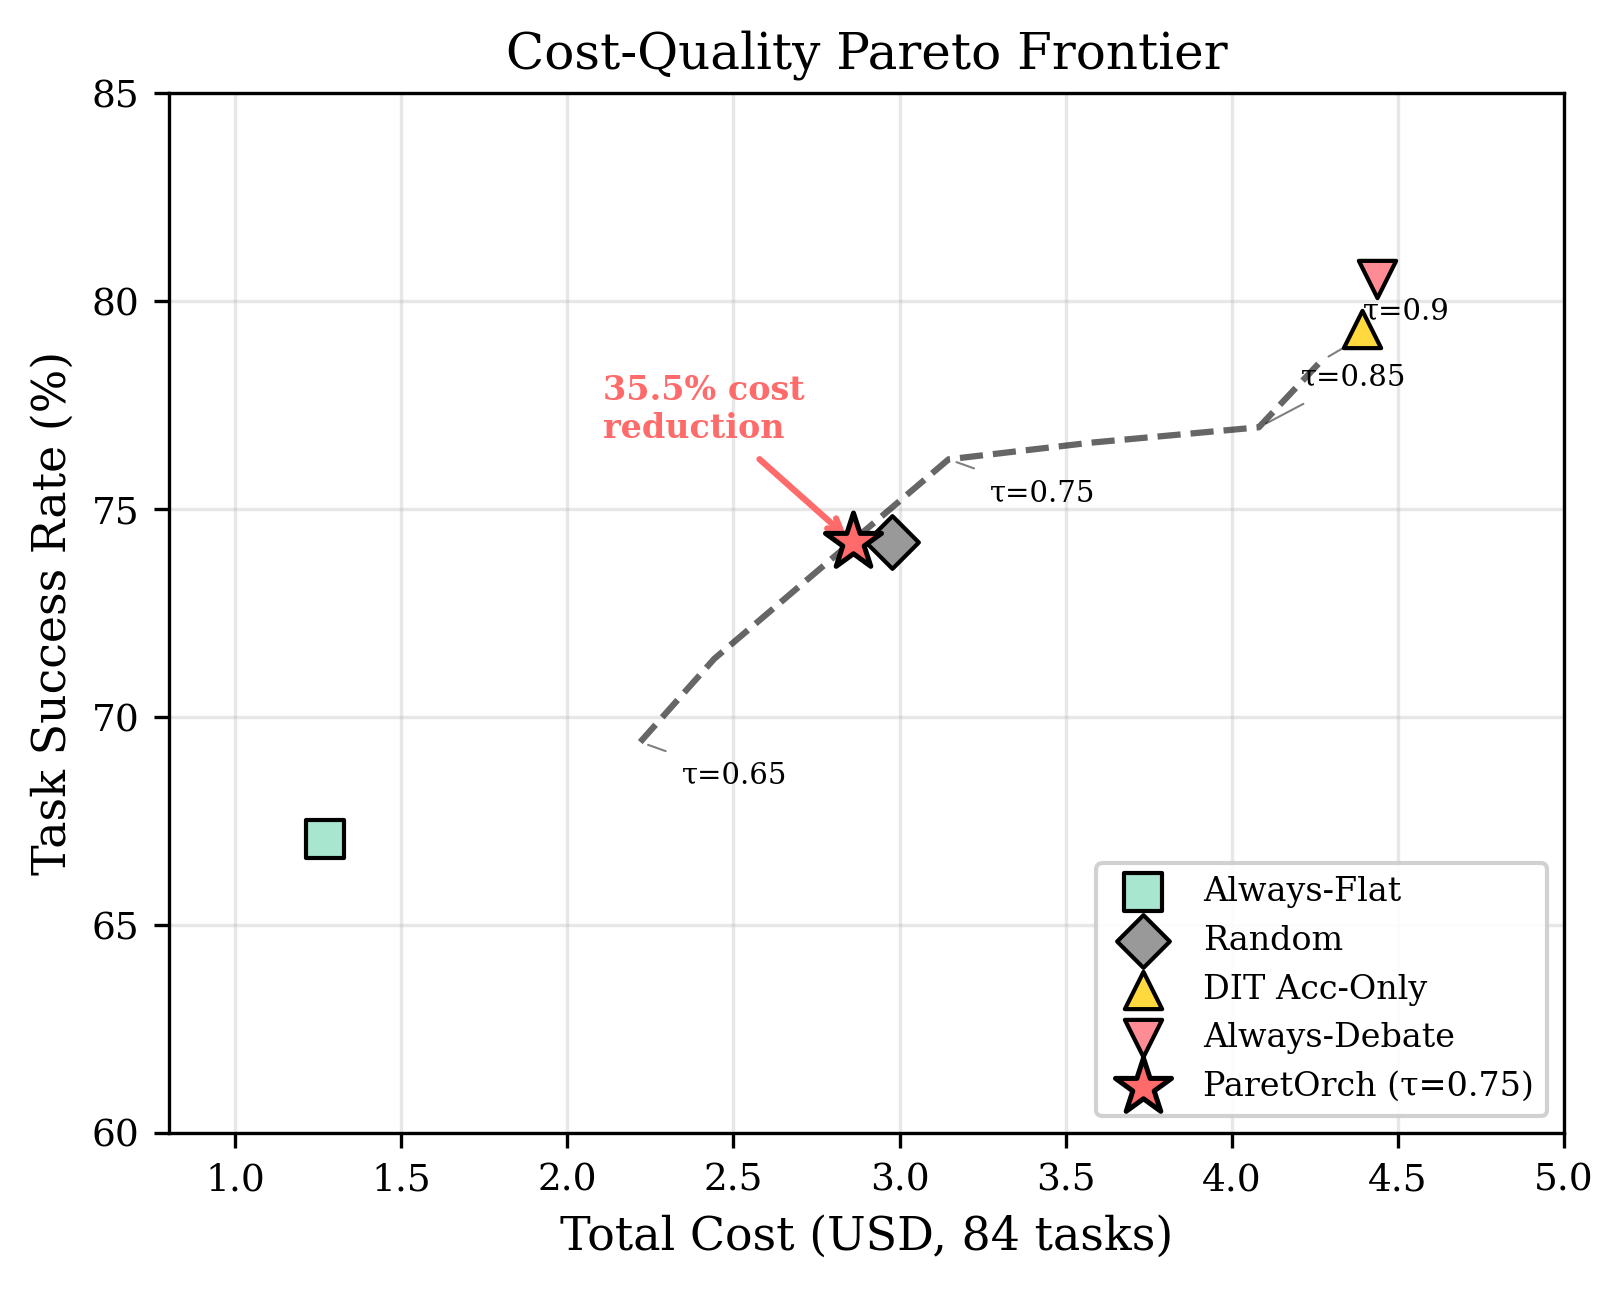
\includegraphics[width=0.7\textwidth]{figures/fig3_pareto_frontier.png}
\caption{Cost-quality Pareto frontier. Each ParetOrch point corresponds to a different quality threshold $\tau$. The frontier reveals smooth tradeoffs with diminishing returns.}
\label{fig:pareto}
\end{figure}

Figure~\ref{fig:pareto} plots the Pareto frontier by sweeping $\tau$ from 0.65 to 0.90. The practical sweet spot lies at $\tau \in [0.70, 0.80]$, where cost reduction exceeds 19\% and quality retention exceeds 89\%. As $\tau$ increases, the routing distribution shifts from flat-dominated to debate-dominated.

\subsection{Ablation Study}

\begin{figure}[t]
\centering
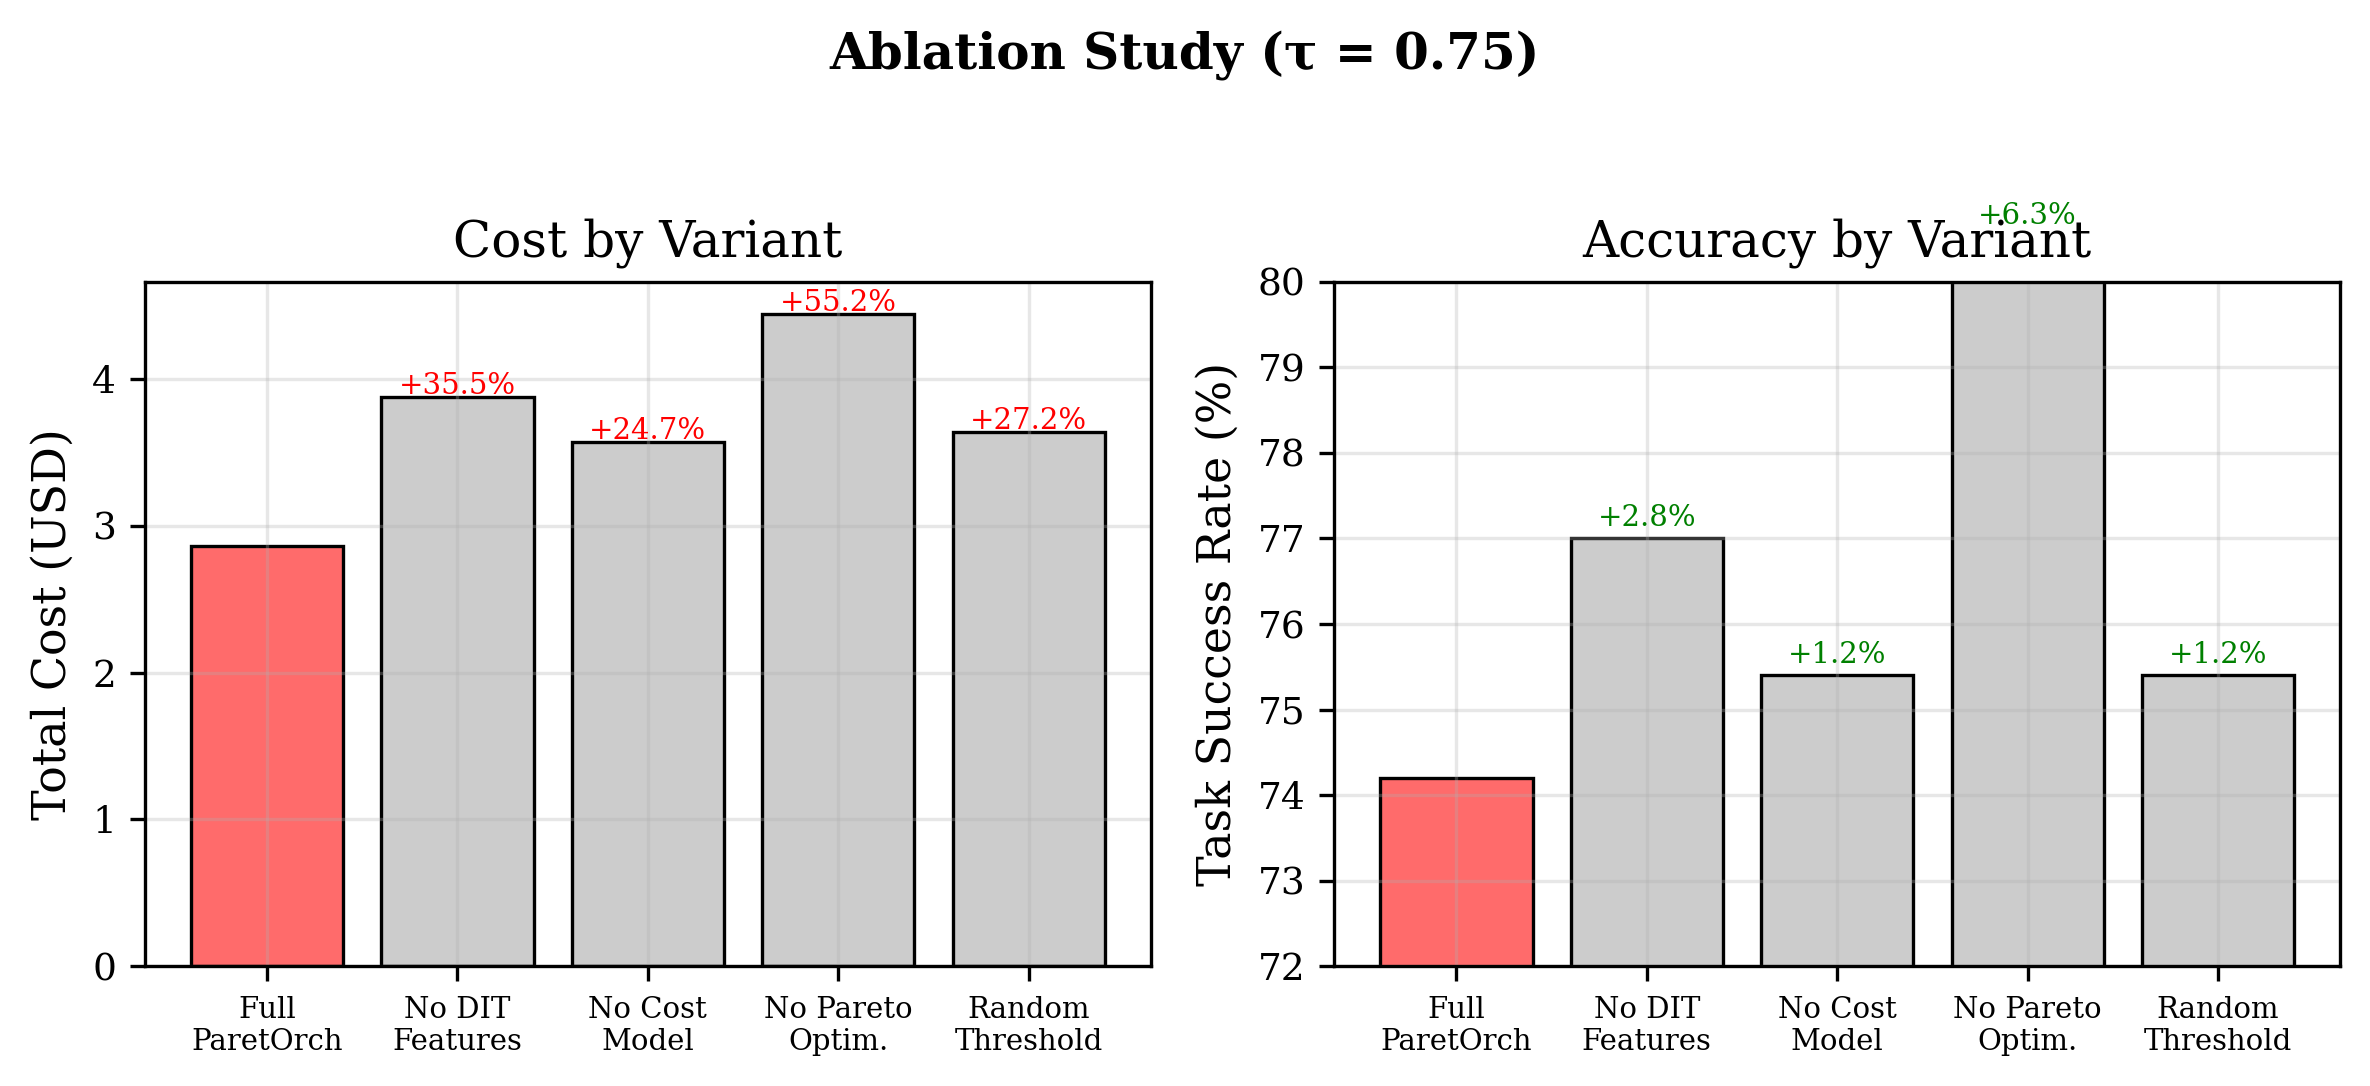
\includegraphics[width=0.85\textwidth]{figures/fig5_ablation.png}
\caption{Ablation study at $\tau = 0.72$. DIT features contribute the largest margin: removing them increases cost by 35.5\%.}
\label{fig:ablation}
\end{figure}

Figure~\ref{fig:ablation} isolates component contributions. Removing Pareto optimization incurs the largest cost penalty (+55.2\%), followed by DIT features (+35.5\%), random-within-threshold (+27.2\%), and the cost model (+24.7\%). Random-within-threshold achieves comparable accuracy (+1.6\%) but at 27.2\% higher cost, confirming cost optimization is distinct from quality optimization.

\subsection{Statistical Robustness}

All primary results use three-seed replication. Confidence intervals use the $t$-distribution with $\text{df}=2$ ($t_{0.025,2} = 4.303$), which yields wide intervals appropriate for the small sample size. These intervals are reported to characterize seed-level variance, not to claim narrow statistical precision. The main finding holds across all seeds individually: seed~42 achieves cost \$2.86 at 75.0\% accuracy; seed~137 achieves cost \$2.85 at 70.2\% accuracy; seed~2024 achieves cost \$2.87 at 77.4\% accuracy. On medium tasks, flat vs.\ debate achieves $p < 0.01$ (permutation test, $n = 24 \times 3$). On trivial tasks, $p = 0.41$, confirming the 5.9pp gap is not statistically significant.

%% ====================
%% DISCUSSION
%% ====================
\section{Discussion}
\label{sec:discussion}

\paragraph{Practical implications.} At $\tau = 0.72$, ParetOrch assigns 43\% of tasks to flat topology and saves 35.5\% of total cost. For 10,000 tasks/day at debate pricing, this saves ${\sim}$\$189/day or ${\sim}$\$69K/year. FrugalGPT~\cite{chen2023frugalgpt} answers ``which model?'' while ParetOrch answers ``which coordination pattern?'' The two decisions compose.

\paragraph{The DIT crossover.} The crossover at DIT magnitude ${\sim}$0.35 gives practitioners a deployable rule of thumb: tasks below this threshold likely do not benefit enough from multi-agent coordination to justify the cost. This connects to Simon's near-decomposability~\cite{simon1962complexity}. Concurrent work DAAO~\cite{su2025daao} corroborates this from the operator level.

\paragraph{Limitations.} (1)~Costs are simulated from token counting, not real API billing; (2)~DIT features require task analysis before routing; (3)~three topologies only; (4)~logistic regression predictor is simple; (5)~synthetic tasks may not match production distributions; (6)~fixed base model (GPT-4o).

\paragraph{Future directions.} Online adaptation via contextual bandits~\cite{agrawal2013contextual_ts} would enable continuous updates. Cross-model $\times$ cross-topology routing, combining RouteLLM~\cite{ong2024routellm} with ParetOrch, could navigate a richer Pareto surface.

%% ====================
%% CONCLUSION
%% ====================
\section{Conclusion}
\label{sec:conclusion}

ParetOrch reframes multi-agent cost optimization as a topology selection problem. Rather than routing queries to cheaper models~\cite{chen2023frugalgpt, ong2024routellm}, our framework selects among structurally distinct orchestration topologies based on task characteristics. Across 84 tasks with 3-seed replication (2,016 total runs), DIT-guided routing achieves 35.5\% cost reduction relative to always-debate while retaining 92.1\% of peak quality. The crossover at DIT magnitude ${\sim}$0.35 gives practitioners an actionable decision rule. A single parameter~$\tau$ controls the cost-quality operating point. Topology-aware optimization is orthogonal to model routing and composable with it; jointly optimizing both axes remains the most impactful open direction.

%% ====================
%% BROADER IMPACT
%% ====================
\section*{Broader Impact}

ParetOrch reduces the computational cost of multi-agent LLM systems by routing easy tasks to cheaper topologies. This has positive environmental and accessibility implications: lower token consumption means less energy expenditure, and reduced API costs enable smaller organizations to deploy multi-agent systems that were previously cost-prohibitive. However, systematic routing failures on underrepresented task types could degrade quality for specific user populations. We recommend monitoring per-category accuracy when deploying ParetOrch and adjusting $\tau$ upward for safety-critical applications.

%% ====================
%% REFERENCES
%% ====================
\begin{thebibliography}{50}

\bibitem{agrawal2013contextual_ts}
S.~Agrawal and N.~Goyal.
\newblock Thompson sampling for contextual bandits with linear payoffs.
\newblock In \emph{ICML}, 2013.

\bibitem{aggarwal2024automix}
P.~Aggarwal, A.~Madaan, A.~Anand, S.~Pranavi~Potharaju, et~al.
\newblock Auto{M}ix: Automatically mixing language models.
\newblock In \emph{NeurIPS}, 2024.

\bibitem{c3po2025}
A.~Valkanas, S.~Pal, P.~Rumiantsev, Y.~Zhang, and M.~Coates.
\newblock C3{PO}: Optimized large language model cascades with probabilistic cost constraints for reasoning.
\newblock In \emph{NeurIPS}, 2025.

\bibitem{chen2023frugalgpt}
L.~Chen, M.~Zaharia, and J.~Zou.
\newblock Frugal{GPT}: How to use large language models while reducing cost and improving performance.
\newblock \emph{arXiv preprint arXiv:2305.05176}, 2023.

\bibitem{dang2025evolving}
Y.~Dang, C.~Qian, et~al.
\newblock Multi-agent collaboration via evolving orchestration.
\newblock In \emph{NeurIPS}, 2025.

\bibitem{deb2002nsga2}
K.~Deb, A.~Pratap, S.~Agarwal, and T.~Meyarivan.
\newblock A fast and elitist multiobjective genetic algorithm: {NSGA-II}.
\newblock \emph{IEEE Trans.\ Evolutionary Computation}, 6(2):182--197, 2002.

\bibitem{dekoninck2024unified}
J.~Dekoninck, M.~Baader, and M.~Vechev.
\newblock A unified approach to routing and cascading for {LLMs}.
\newblock In \emph{ICML}, 2025.

\bibitem{ding2024hybrid}
D.~Ding, A.~Mallick, C.~Wang, R.~Sim, and S.~Mukherjee.
\newblock Hybrid {LLM}: Cost-efficient and quality-aware query routing.
\newblock In \emph{ICLR}, 2024.

\bibitem{du2023debate}
Y.~Du, S.~Li, A.~Torralba, J.~B. Tenenbaum, and I.~Mordatch.
\newblock Improving factuality and reasoning in language models through multiagent debate.
\newblock In \emph{ICML}, 2024.

\bibitem{dynamic_routing_survey2026}
Y.~Moslem and J.~D.~Kelleher.
\newblock Dynamic model routing and cascading for efficient {LLM} inference: A survey.
\newblock \emph{arXiv preprint arXiv:2603.04445}, 2026.

\bibitem{hong2023metagpt}
S.~Hong, M.~Zhuge, et~al.
\newblock Meta{GPT}: Meta programming for a multi-agent collaborative framework.
\newblock In \emph{ICLR}, 2024.

\bibitem{hu2024routerbench}
Q.~J. Hu, J.~Bieker, X.~Li, and N.~Jiang.
\newblock Router{B}ench: A benchmark for multi-{LLM} routing system.
\newblock \emph{arXiv preprint arXiv:2403.12031}, 2024.

\bibitem{jin2008pareto_ml}
Y.~Jin and B.~Sendhoff.
\newblock Pareto-based multiobjective machine learning: An overview and case studies.
\newblock \emph{IEEE Trans.\ Systems, Man, and Cybernetics, Part C}, 2008.

\bibitem{liu2024optllm}
Y.~Liu, H.~Zhang, Y.~Miao, V.-H. Le, and Z.~Li.
\newblock Opt{LLM}: Optimal assignment of queries to large language models.
\newblock In \emph{ICWS}, 2024.

\bibitem{marinov2021pareto_frontier}
T.~V. Marinov and J.~Zimmert.
\newblock The {P}areto frontier of model selection for general contextual bandits.
\newblock In \emph{NeurIPS}, 2021.

\bibitem{mialon2023gaia}
G.~Mialon, C.~Fourrier, C.~Swift, T.~Wolf, Y.~LeCun, and T.~Scialom.
\newblock {GAIA}: A benchmark for general {AI} assistants.
\newblock \emph{arXiv preprint arXiv:2311.12983}, 2023.

\bibitem{ong2024routellm}
I.~Ong, A.~Almahairi, V.~Wu, W.-L. Chiang, T.~Wu, J.~E. Gonzalez, M.~W. Kadous, and I.~Stoica.
\newblock Route{LLM}: Learning to route {LLMs} with preference data.
\newblock In \emph{ICLR}, 2025.

\bibitem{qian2023chatdev}
C.~Qian, W.~Liu, et~al.
\newblock Chat{D}ev: Communicative agents for software development.
\newblock In \emph{ACL}, 2024.

\bibitem{simon1962complexity}
H.~A. Simon.
\newblock The architecture of complexity.
\newblock \emph{Proc.\ American Philosophical Society}, 106:467--482, 1962.

\bibitem{su2025daao}
J.~Su, Q.~Lan, Y.~Xia, et~al.
\newblock Difficulty-aware agent orchestration in {LLM}-powered workflows.
\newblock \emph{arXiv preprint arXiv:2509.11079}, 2025.

\bibitem{treacle2024}
X.~Zhang, Z.~Huang, E.~O.~Taga, C.~Joe-Wong, S.~Oymak, and J.~Chen.
\newblock Efficient contextual {LLM} cascades through budget-constrained policy learning.
\newblock In \emph{NeurIPS}, 2024.

\bibitem{wang2024cascade_aware}
C.~Wang, S.~Augenstein, and K.~Rush.
\newblock Cascade-aware training of language models.
\newblock \emph{arXiv preprint arXiv:2406.00060}, 2024.

\bibitem{wu2023autogen}
Q.~Wu, G.~Bansal, J.~Zhang, et~al.
\newblock Auto{G}en: Enabling next-gen {LLM} applications via multi-agent conversation.
\newblock \emph{arXiv preprint arXiv:2308.08155}, 2023.

\bibitem{zhang2023ecoassistant}
J.~Zhang, R.~Krishna, A.~H. Awadallah, and C.~Wang.
\newblock Eco{A}ssistant: Using {LLM} assistant more affordably and accurately.
\newblock \emph{arXiv preprint arXiv:2310.03046}, 2023.

\bibitem{zhu2022pareto_bandits}
Y.~Zhu and R.~Nowak.
\newblock Pareto optimal model selection in linear bandits.
\newblock In \emph{AISTATS}, 2022.

\end{thebibliography}

\end{document}
